\documentclass[a4paper,8pt]{beamer}
\usepackage[slovene]{babel}
\usepackage[utf8]{inputenc}
\usepackage[T1]{fontenc}
\usepackage{lmodern}
\usepackage{amsmath}
\usepackage{array}
\usepackage{tikz}

%\setbeamertemplate{navigation symbols}{}

\usetheme{Berlin}
\beamertemplatenavigationsymbolsempty
\setbeamertemplate{headline}{}
\usecolortheme{default}
\useinnertheme{rounded}
\useoutertheme{infolines}

\usepackage{palatino}
\usefonttheme{serif}

\setbeamertemplate{navigation symbols}{}

\usepackage{subfig}
\usepackage{graphicx}
\graphicspath{{./slike/}}


\newcommand{\R}{\mathbb R}
\newcommand{\N}{\mathbb N}
\newcommand{\Z}{\mathbb Z}

\newtheorem{definicija}{Definicija}
\newtheorem{izrek}{Izrek}
\newtheorem{lema}{Lema}
\newtheorem{trditev}{Trditev}
\newtheorem{posledica}{Posledica}
\newtheorem{primer}{Primer}

\newcommand{\tbf}{\textbf}

\title{Gregoryjeve krpe}
\author{Klara Kersnik in Meta Trdin} % \\ ndlkndl}
%\author[My name]{\textbf {Directed by: my name\\ \footnotesize Supervised by: first name, second name}}
\institute[FMF]{Fakulteta za matematiko in fiziko}
\date{}




\begin{document}

\begin{frame}
\maketitle
\end{frame}

\begin{frame}{Vsebina}

\begin{enumerate}
	\item Uvod
	\item Metoda Chiyokura in Kimura
	\item Gregoryjeve krpe
	\begin{enumerate}
		\item Kvadratne Gregoryjeve krpe
		\item Trikotne Gregoryjeve krpe
	\end{enumerate}
\end{enumerate}

\end{frame}

\begin{frame}{Uvod}
\begin{itemize}
	\item ponovimo definicijo G1 zveznosti
\end{itemize}

\begin{figure}[h]
	\centering
	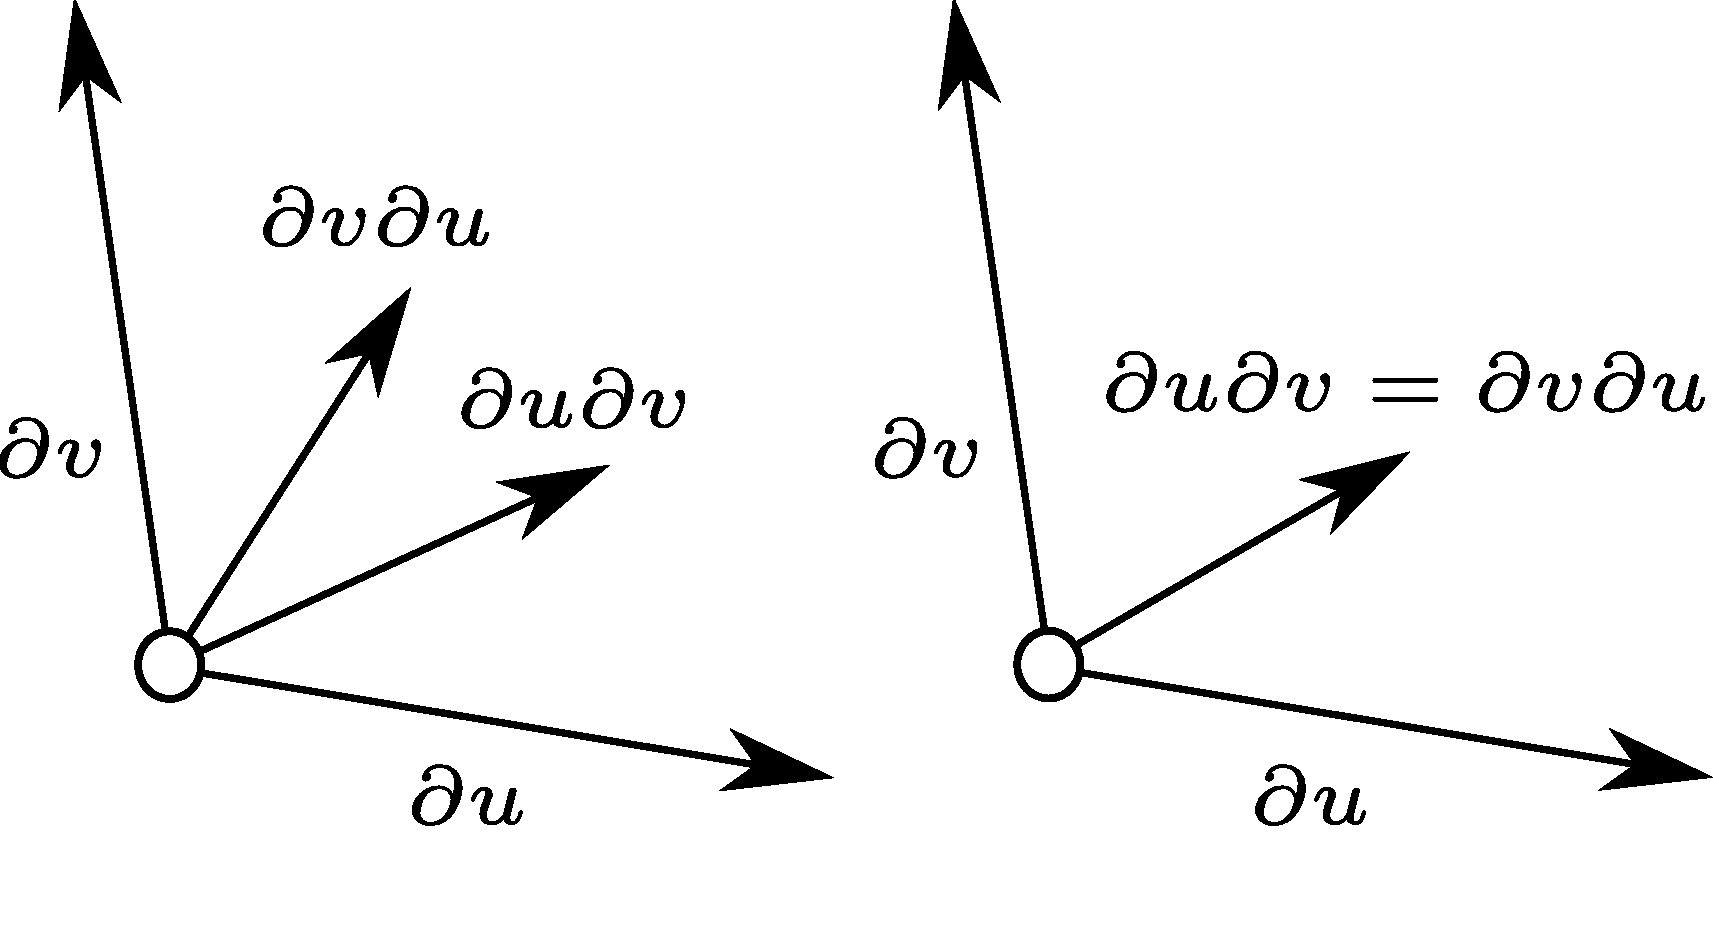
\includegraphics[width=6cm]{mesani_odvodi_ob.jpg}
	\caption{Mešani odvodi}
\end{figure}
\end{frame}


\begin{frame}{Metoda Chyokura in Kimura}
	
\end{frame}
\begin{frame}
	\begin{figure}[h]
		\centering
		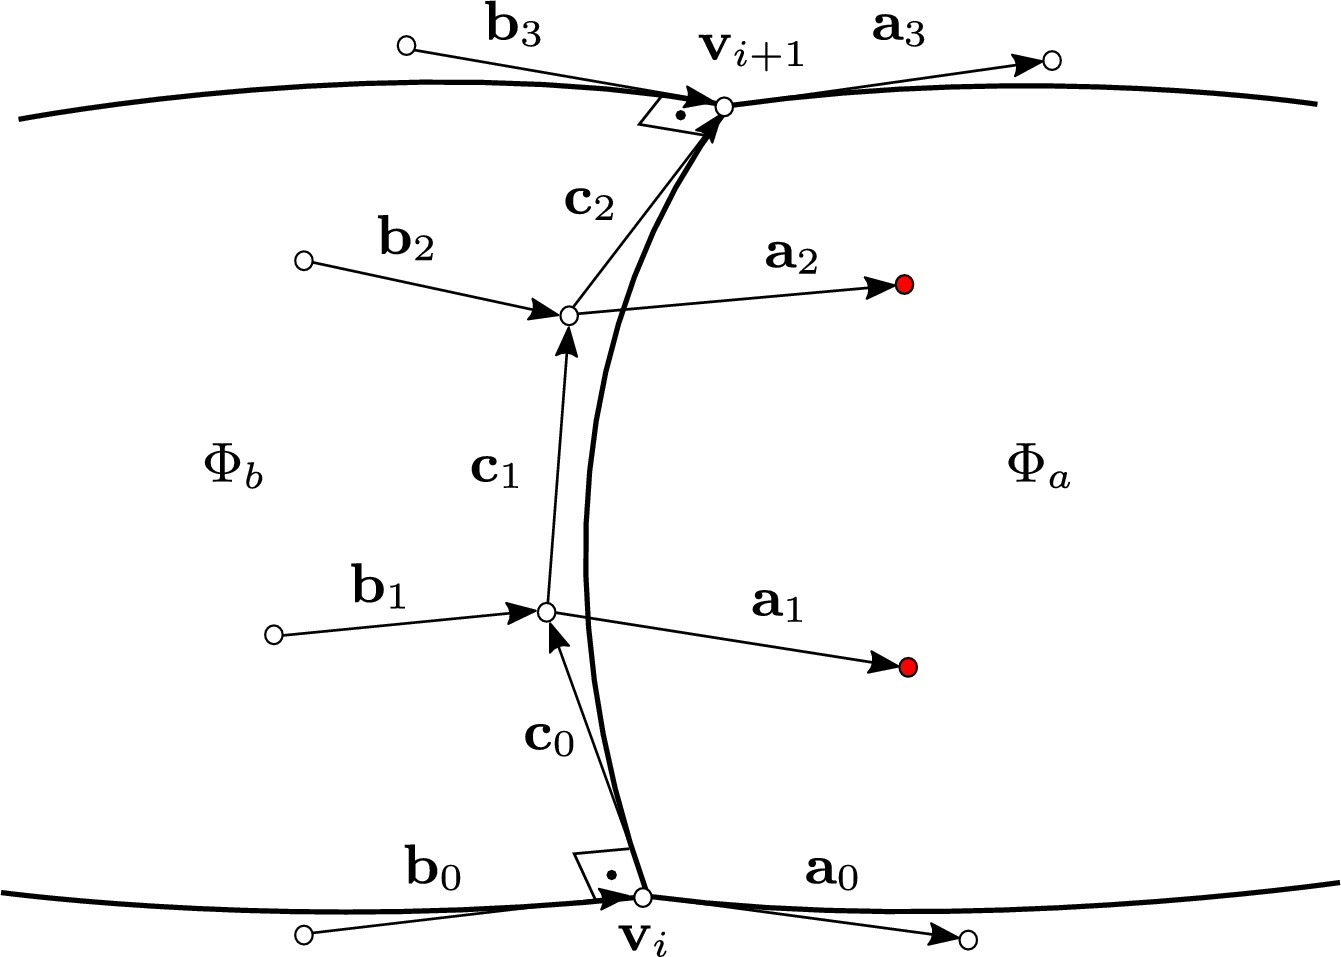
\includegraphics[width=6cm]{metoda_CinK.jpg}
		\caption{Metoda Chiyokura in Kimura}
	\end{figure}
\end{frame}

\section{Gregoryjeve krpe}
\begin{frame}{Kvadratne Gregoryjeve krpe}


Konstrukcija
\begin{itemize}
	\item Želimo parametrizirati ploskev v prostoru, da bo imela $G1$ zveznost, ko jo bomo zlepili
	\item domena $[0,1] \times [0,1]$
	\item Podane imamo $4$ robne krivulje: bezierjeve krivulje reda $3$
	\item Na vsakem robu uporabimo metodo Chyyokura in Kimura (dobimo $2 \cdot 4 = 8$ točk)
	\item Nastopi twist compatibility problem. Tukaj si pomagamo z racionalnii funkcijami:
		\begin{align*}
		\textbf{b}_{11} &=  \frac{v \textbf{b}_{11,u_0}+u\tbf{b}_{11,v_0}}{u +v} \\
		\tbf{b}_{21} &= \frac{(1-v) \tbf{b}_{21,u_0}+u\tbf{b}_{21,v_1}}{(1-v)+u} \\
		\tbf{b}_{12} &= \frac{v \tbf{b}_{12,u_1}+(1-u)\tbf{b}_{12,v_0}}{v+(1-u)} \\
		\tbf{b}_{22} &= \frac{(1-v) \tbf{b}_{22,u_1}+(1-u)\tbf{b}_{22,v_1}}{(1-u)+(1-v)} 
		\end{align*}
\end{itemize}
	
\end{frame}
\begin{frame}
	\begin{figure}[h]
		\centering
		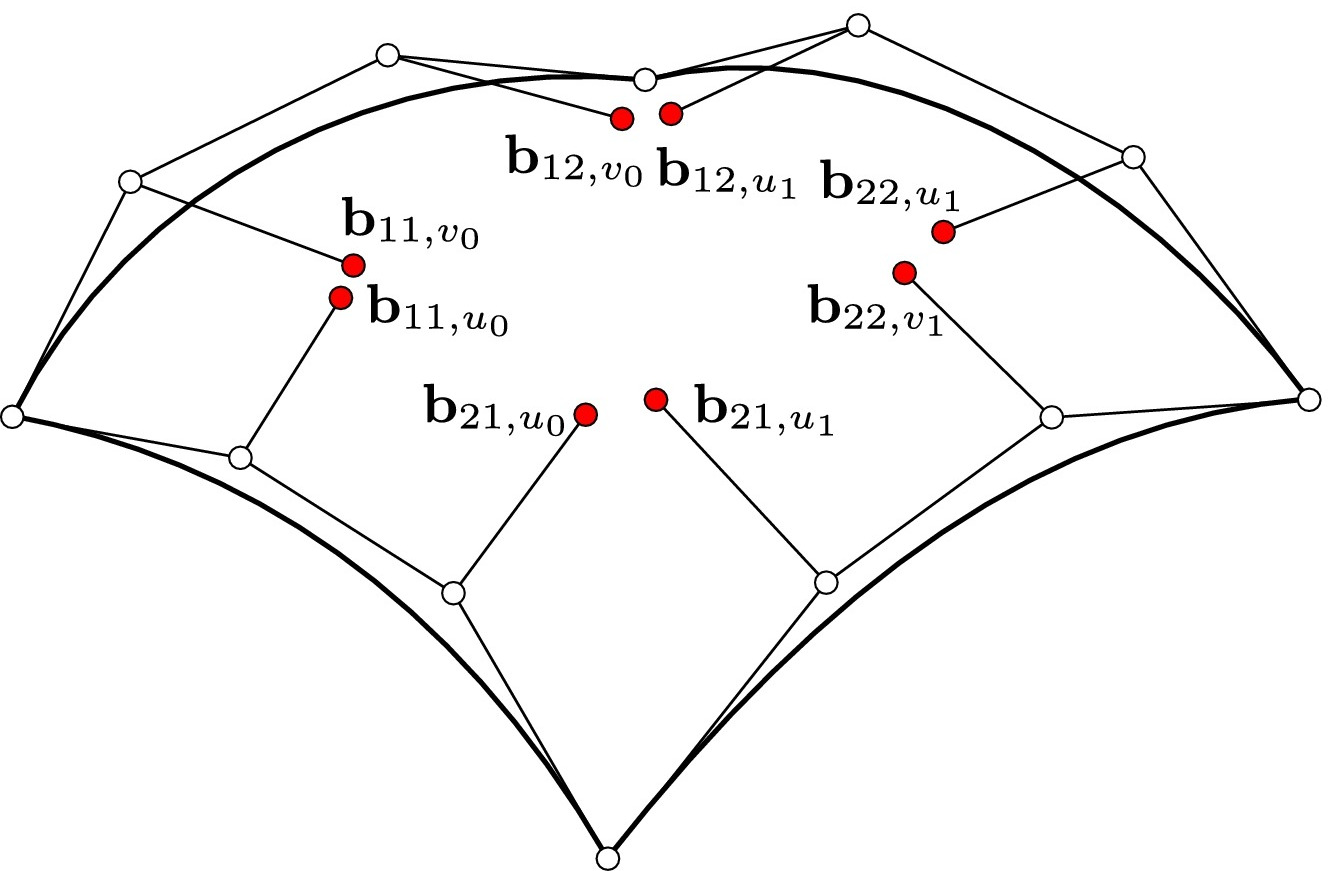
\includegraphics[width=10cm]{gregory_krpe_kvadratna.jpg}
		\caption{Kvadratna Gregoryjeva krpa}
	\end{figure}
\end{frame}

\begin{frame}{Trikotne Gregoryjeve krpe}
	\begin{itemize}
		\item trikotna domena
		\item 3 kubične bezierjeve krivulje na robu
		\item Uporabimo metodo Chyyokura in Kimura (dobimo $2 \cdot 3 = 6$ točk)
		\item na posameznem paru uporabim racionalno funkcijo da dobimo 3 notranje točke
		\item kubična bezierjeva krpa ima le eno kontrolno točko ki ni robna, kvadratna pa ima 3 kar nam v tem primeru bolj ustreza. Zato moramo še robnim krivuljam zvišati stopnjo.
		\item Posamezen par združimo v eno točko:
		\begin{align*}
		\tbf{b}_{211} &= \frac{(1-w)v \tbf{b}_{211,uv}+(1-v)w\tbf{b}_{211,v_1}}{(1-w)v+(1-v)w} \\
		\tbf{b}_{121} &= \frac{(1-w)u \tbf{b}_{121,uv}+(1-u)v\tbf{b}_{121,vw}}{(1-w)u+(1-u)w} \\
		\tbf{b}_{112} &= \frac{(1-u)v \tbf{b}_{112,vw}+(1-v)u\tbf{b}_{112,uw}}{(1-u)v+(1-v)u} 
		\end{align*}
	\end{itemize}
\end{frame}
\begin{frame}
	\begin{figure}[h]
		\centering
		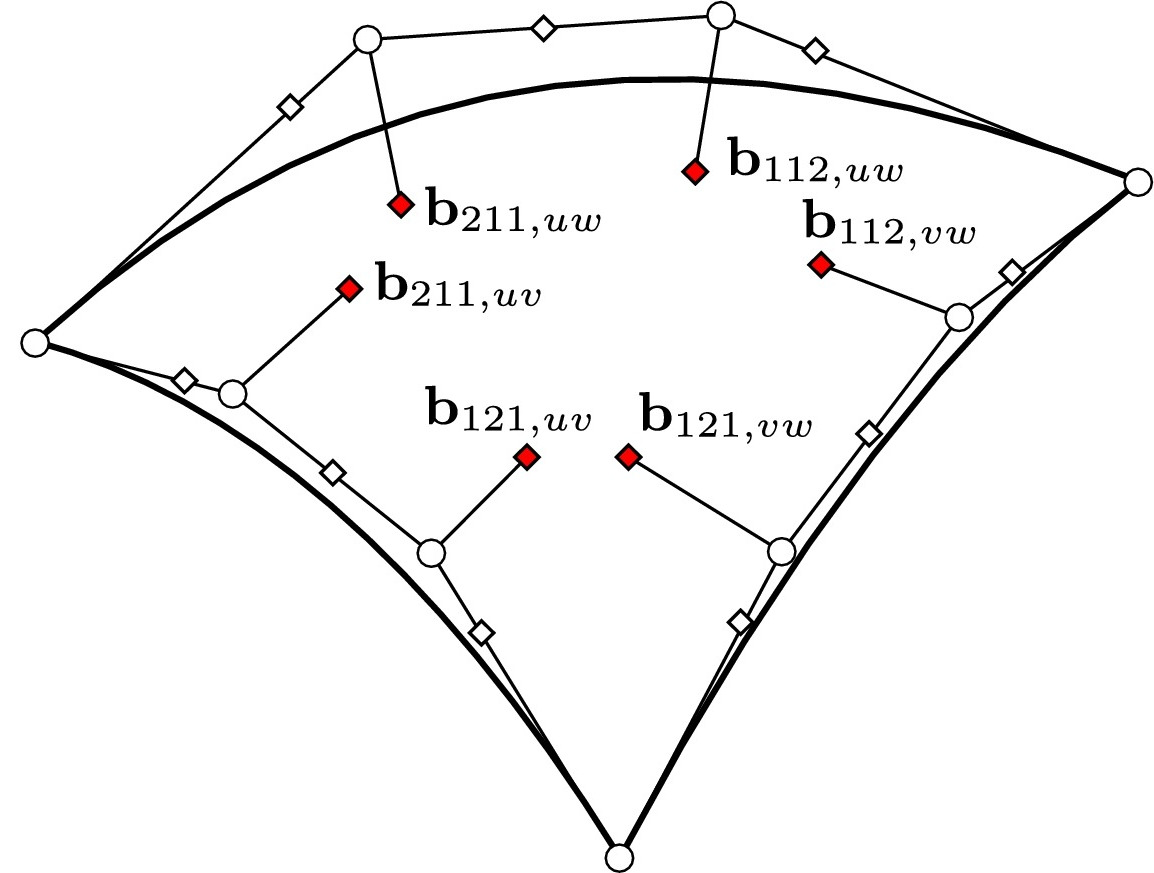
\includegraphics[width=10cm]{gregory_krpe_trikotna.jpg}
		\caption{Trikotna Gregoryjeva krpa}
	\end{figure}
\end{frame}




















\end{document}